
\begin{figure}
  \centering
  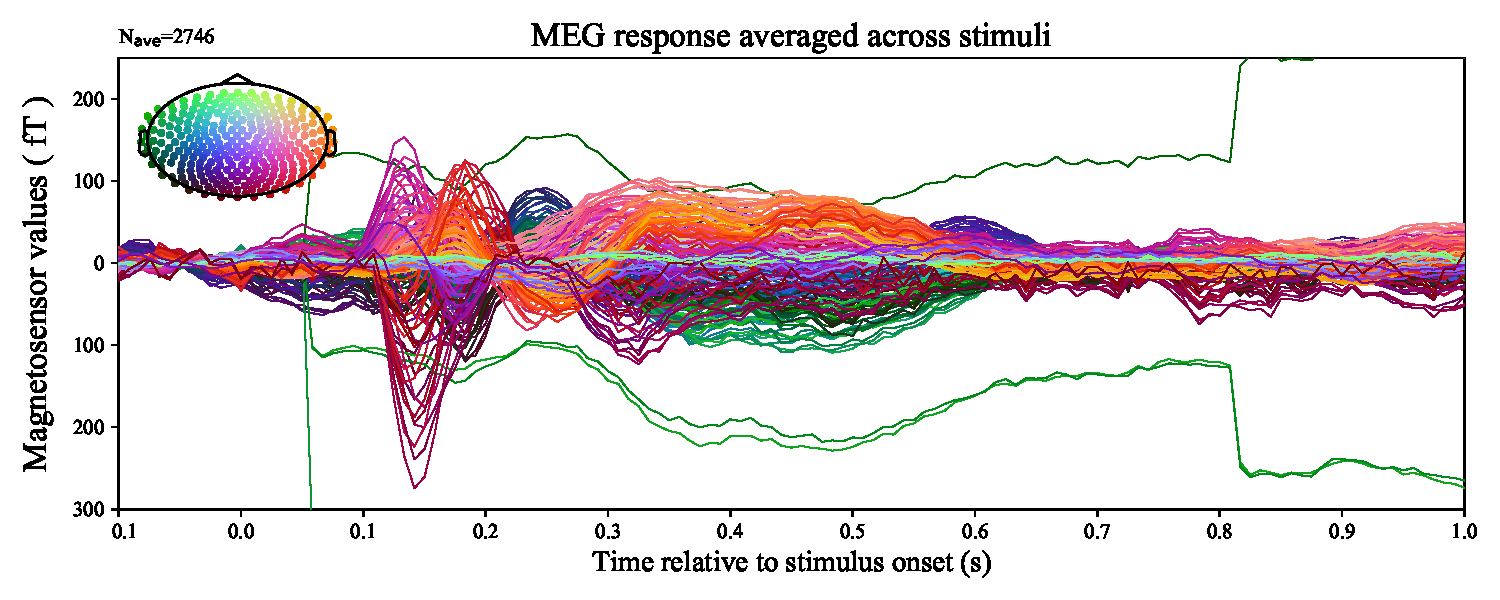
\includegraphics[width=\textwidth, trim=0cm 0cm 0cm 0cm, clip=True]{figures/meg_sensors.pdf}
  \caption{Magnetosensor response (femtoteslas fT) averaged across words for the first subject. The color coding corresponds to the positions of the sensors on the head as shown on the top-left diagram. The diverging curves correspond to artifacts in the MEG data.}
  \label{fig:megavg}
\end{figure}
